%%%%%%%%%%%%%%%%%%%%%%%%%%%%%%%%%%%%%%%%%%%%%%%%%%%%%%%%%%%%%%%%%%%%%%%%%%%%%%%%
% Template for USENIX papers.
%
% History:
%
% - TEMPLATE for Usenix papers, specifically to meet requirements of
%   USENIX '05. originally a template for producing IEEE-format
%   articles using LaTeX. written by Matthew Ward, CS Department,
%   Worcester Polytechnic Institute. adapted by David Beazley for his
%   excellent SWIG paper in Proceedings, Tcl 96. turned into a
%   smartass generic template by De Clarke, with thanks to both the
%   above pioneers. Use at your own risk. Complaints to /dev/null.
%   Make it two column with no page numbering, default is 10 point.
%
% - Munged by Fred Douglis <douglis@research.att.com> 10/97 to
%   separate the .sty file from the LaTeX source template, so that
%   people can more easily include the .sty file into an existing
%   document. Also changed to more closely follow the style guidelines
%   as represented by the Word sample file.
%
% - Note that since 2010, USENIX does not require endnotes. If you
%   want foot of page notes, don't include the endnotes package in the
%   usepackage command, below.
% - This version uses the latex2e styles, not the very ancient 2.09
%   stuff.
%
% - Updated July 2018: Text block size changed from 6.5" to 7"
%
% - Updated Dec 2018 for ATC'19:
%
%   * Revised text to pass HotCRP's auto-formatting check, with
%     hotcrp.settings.submission_form.body_font_size=10pt, and
%     hotcrp.settings.submission_form.line_height=12pt
%
%   * Switched from \endnote-s to \footnote-s to match Usenix's policy.
%
%   * \section* => \begin{abstract} ... \end{abstract}
%
%   * Make template self-contained in terms of bibtex entires, to allow
%     this file to be compiled. (And changing refs style to 'plain'.)
%
%   * Make template self-contained in terms of figures, to
%     allow this file to be compiled. 
%
%   * Added packages for hyperref, embedding fonts, and improving
%     appearance.
%   
%   * Removed outdated text.
%
%%%%%%%%%%%%%%%%%%%%%%%%%%%%%%%%%%%%%%%%%%%%%%%%%%%%%%%%%%%%%%%%%%%%%%%%%%%%%%%%

\documentclass[letterpaper,twocolumn,10pt]{article}
\usepackage{usenix2019_v3}

% to be able to draw some self-contained figs
\usepackage{hyperref}
\usepackage{tikz}
\usepackage{amsmath}
\usepackage{tabularx}
\usepackage{float}
\usepackage{booktabs}

%-------------------------------------------------------------------------------
\begin{document}
%-------------------------------------------------------------------------------
\date{}
\title{\Large Adversarial Obfuscation for Domain Fronting}
\author{
{\rm Steven R. Sheffey}\\
Middle Tennessee State University
\and
{\rm Ferrol Aderholdt}\\
Middle Tennessee State University
} % end author

\maketitle

%-------------------------------------------------------------------------------
\begin{abstract}
%-------------------------------------------------------------------------------
% Your abstract text goes here. Just a few facts. Whet our appetites.
% Not more than 200 words, if possible, and preferably closer to 150.
As the becomes more important as a source of information, internet censorship has become more pervasive. Tor aims to circumvent censorship, but adversaries are capable of blocking Tor traffic. Pluggable transports are used to obfuscate tor traffic to circumvent this. Meek uses domain fronting to emulate benign and trusted HTTPS traffic, with the hope that adversaries will avoid blocking it in order to avoid the collateral damage of blocking a reputable website. However, attacks using machine learning to differentiate domain-fronted traffic from regular HTTPS traffic pose a threat to the effectiveness of domain fronting. We propose the use of adversarial machine learning to model and reduce this threat.
\end{abstract}


%-------------------------------------------------------------------------------
\section{Introduction}
%-------------------------------------------------------------------------------
Meek provides excellent protection against metadata-based DPI attacks and resilience to censorship by hiding traffic inside encrypted HTTPS flows to reputable websites. However, due to its distinct activity pattern, it can be trivially identified by machine learning algorithms analyzing its traffic patterns.

Adversarial neural networks are powerful for modeling scenarios in which one party is trying to classify data, and another party is trying to produce fake or modified data that can fool the classifier. The result of training an adversarial model is a discriminator that is somewhat resilient to fakes, and a generator that can generate fake data, or modify data in a way that changes its perceived class. We believe that adversarial models can model internet censorship and help provide obfuscators such as Meek information to reduce its detectability.
\nocite{*}


%-------------------------------------------------------------------------------
\section{Background}
%-------------------------------------------------------------------------------

\subsection{Censorship}
\begin{itemize}
    \item Internet censorship has become pervasive (china, iran, saudi arabia, russia, etc)
    \item The Tor network is used to circumvent internet censorship
    \item Censors have blocked Tor
\end{itemize}
\subsection{Obfuscation}
Obfuscators are used to circumvent protocol censorship or increase privacy. Tor uses Pluggable Transports
\subsubsection{Forms of Obfuscation}

\begin{itemize}
    \item Randomization (obfsproxy, scramblesuit)
    \item Mimicry (Skypemorph, Marionette, FTE)
    \item Tunneling (Meek)
    \item Traffic shaping, chaff
    \item TODO: snowflake, other newer obfuscators
\end{itemize}
TODO: go into detail about meek

\subsubsection{Attacks against Obfuscation}
\begin{itemize}
    \item Syntactic/Semantic (badly obfuscated traffic doesn't make sense semantically in its transformed protocol)
    \item Entropy
    \item Traffic statistical analysis
    \item TODO: others
\end{itemize}

TODO: go into detail about statistical analysis/machine learning

Wang et al.~\cite{Wang:2015:STN:2810103.2813715} were able to identify Meek traffic with a FPR (false positive rate) of 0.0002 on meek-amazon and 0.00006 on meek-google. This indicates that traffic analysis attacks using machine learning pose a major threat to traffic obfuscation and anti-censorship efforts.

%-------------------------------------------------------------------------------
\section{Related Work}
TODO: talk move about wang et al

TODO: find more papers identifying tor with machine learning

TODO: talk about the other adversarial transformation paper

\section{Data Collection}
We implement a framework that allows for reproducible, parallel generation of packet captures for HTTPS traffic with and without tor and pluggable transports.
\subsection{Framework}
\begin{figure}[H]
    \centering
    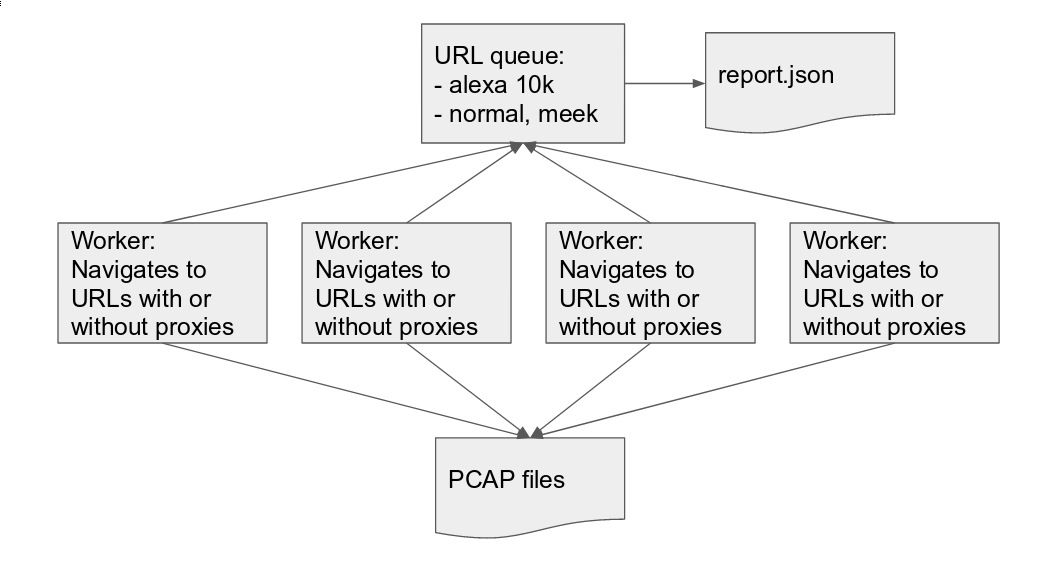
\includegraphics[width=0.5\textwidth]{figures/data-collection-architecture}
    \caption{\label{fig:data-collection-architecture} Architecture of data collection containers} 
\end{figure}
The data collection framework is composed of two types of containers: \textit{URL Queue}, a work queue containing URLs and proxy types, and \textit{Workers} that navigate to URLs using the given proxy and recort packet captures. Each type of container is run using Docker. Docker allows for reproducibility of the data collection process, parallelism, and isolation of the traffic captures by each worker. Each worker requests a piece of work from the URL queue. The worker then starts \texttt{tcpdump} to record all network traffic. If the work type requires startng TOR, then TOR is started with the given pluggable transport. In this work, we use \texttt{meek-azure} to tunnel our TOR traffic through Meek. Because the first start of TOR downloads and caches a large amount of data, we mark the first Tor work on each worker to allow it to be potentially accounted for. Once the TOR process has been started, we start Firefox using Selenium. After starting the browser, if TOR is used, we wait 10 seconds to ensure the pluggable transport has been properly initialized. Then, we use Selenium to navigate to the webpage. Because some webpages are constantly downloading content in a way that prevents Selenium from marking the page as finished loading, we wait for either common tag to appear (\texttt{<script>}) or {TODO} seconds to pass. After the page has been loaded, the worker shuts down the browser, TOR, and TCPDUMP. The worker then sends a report to the URL queue service containing information about the work done, and the filename of the \texttt{pcap} file. The overall architecture of the data collection framework is shown in Figure~\ref{fig:data-collection-architecture}.
\subsection{Datasets}
Each of our datasets contains packet captures for navigating to the top 10000 websites of the Alexa top 1M both without any proxies, and through Tor over Meek. We collect datasets from a home wired network ($H_{normal}$, $H_{meek}$), a university wired network ($U_{normal}$, $U_{meek}$), and an AWS \texttt{m5.2xlarge} instance ($A_{normal}$, $A_{meek}$).
\subsection{Feature Extraction}
In order to extract packet-level features, we use \textit{BRO}, a DPI engine, to generate a set of connections for each \texttt{PCAP}. Using this list of connections, we use a program to associate packets with connections based on source IP, destination IP, source port, destination port, and timestamp. For each HTTPS connection, we sort the packets by timestamp, and then extract  features from each packet. The features extracted are TCP payload size, and time since the last packet of the same direction.

The values for all connections in a \texttt{pcap} are aggregated into a histogram with logarithmic bins. Logarithmic bins are used because much more information is found in the smaller packet sizes and inter-arrival times than larger ones.

\begin{figure}[H]
    \centering
    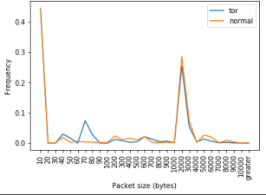
\includegraphics[width=0.4\textwidth]{figures/initial-features-packet-size}
    \caption{\label{fig:initial-features-packet-size} Averaged packet sizes from dataset H} 
\end{figure}
\begin{figure}[H]
    \centering
    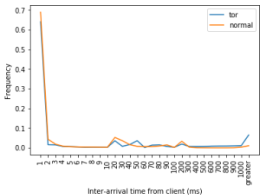
\includegraphics[width=0.4\textwidth]{figures/initial-features-iaf}
    \caption{\label{fig:initial-features-iaf} Averaged inter-arrival time (from client) from dataset H} 
\end{figure}
\begin{figure}[H]
    \centering
    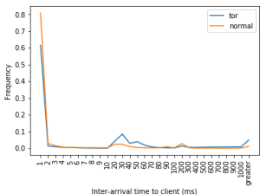
\includegraphics[width=0.4\textwidth]{figures/initial-features-iat}
    \caption{\label{fig:initial-features-iaf} Averaged inter-arrival time (to client) from dataset H} 
\end{figure}
TODO: explain feature these graphs.
\section{Adversarial Model}
\subsection{Architecture}
\begin{figure*}[ht!]
    \centering
    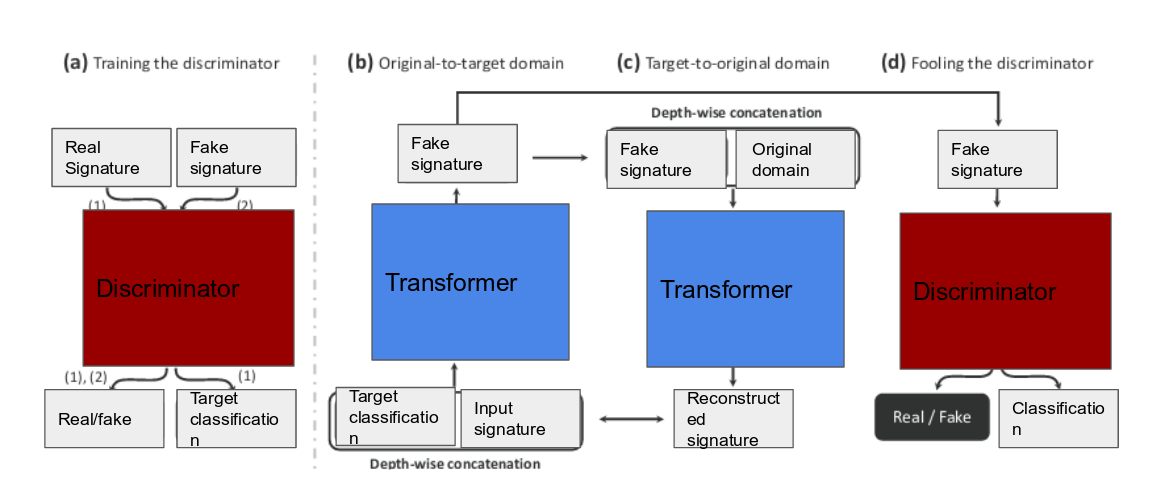
\includegraphics[width=\textwidth]{figures/stargan-architecture}
    \caption{\label{fig:stargan-architecture} Architecture of our adapted version of StarGAN} 
\end{figure*}
We use StarGAN~\cite{Choi_2018_CVPR} as a basis for obfuscation. StarGAN allows for adversarial transformation through application of a variety of features, though for this model, we only use a binary set of features (Meek or normal). Additionally, StarGAN performs well on datasets from multiple domains, which has potential applications in transforming obfuscated traffic of multiple types or locations.

Compared to StarGAN, we make some modifications to the model process. In our model, rather than complex convolutional neural networks, we use simple fully connected neural networks in our discriminator and generator. In addition, to ensure that minimal perturbation is made to the signatures, we add an additional constraint to StarGAN's generator loss function that minimizes mean absolute difference between the transformed signature and the input signature.

The classifier used to evaluate the model's efficiency is a basic feed forward neural network, with similar architecture to the discriminator. We also use a random forest classifier in the classification stages, to provide a measure of transformation effect on models that are not neural networks.

\subsection{Training and Evaluation}
The training and evaluation process is composed of 5 steps
\begin{enumerate}
    \item Train the GAN (Discriminator and Transformer)
    \item Train classifiers
    \item Evaluate correctness of classifier
    \item Evaluate correctness of classifier on transformed traffic
    \item Evaluate correctness of classifier on transformed traffic with flipped labels
\end{enumerate}
In order to validate this process, we split the dataset into three sets:
\begin{itemize}
    \item 50\% GAN training set
    \item 30\% Classifier training set
    \item 20\% Classifier training set
\end{itemize}
We shuffle the dataset randomly and then use K-fold validation to perform our training and evaluation process on all 6 orderings of these dataset splits.


%-------------------------------------------------------------------------------
\section{Results}
%-------------------------------------------------------------------------------
Our models succeded at fooling all tested classifiers with minimal perturbation
\begin{figure}[H]
    \centering
    \begin{tabularx}{0.5\textwidth}{ X X X X }
      \toprule
        & Baseline & Transformed & Transformed \& flipped class \\
      \midrule
      Classifier  & 0.99  & 0.3  & 0.99  \\
      Discriminator & 0.99  & 0.3  & 0.99  \\
      Random Forest & 0.99  & 0.3  & 0.99  \\
      \bottomrule
    \end{tabularx}
    \caption{\label{fig:results-pr-auc-h} Effect of transformer on PR-AUC on dataset H} 
\end{figure}
\begin{figure}[H]
    \centering
    \begin{tabularx}{0.5\textwidth}{ X X X X }
      \toprule
        & Baseline & Transformed & Transformed \& flipped class \\
      \midrule
      Classifier  & 0.99  & 0.3  & 0.99  \\
      Discriminator & 0.99  & 0.3  & 0.99  \\
      Random Forest & 0.99  & 0.3  & 0.99  \\
      \bottomrule
    \end{tabularx}
    \caption{\label{fig:results-pr-auc-u} Effect of transformer on PR-AUC on dataset U} 
\end{figure}
\begin{figure}[H]
    \centering
    \begin{tabularx}{0.5\textwidth}{ X X X X }
      \toprule
        & Baseline & Transformed & Transformed \& flipped class \\
      \midrule
      Classifier  & 0.99  & 0.3  & 0.99  \\
      Discriminator & 0.99  & 0.3  & 0.99  \\
      Random Forest & 0.99  & 0.3  & 0.99  \\
      \bottomrule
    \end{tabularx}
    \caption{\label{fig:results-pr-auc-a} Effect of transformer on PR-AUC on dataset A} 
\end{figure}
%-------------------------------------------------------------------------------
\section{Conclusions}
%-------------------------------------------------------------------------------
Our results indicate that adversarial neural networks show promise in identifying and modifying statistical signatures of traffic that could be used to make the traffic more identifiable. Transformations performed by the neural network validate previous work's conclusions that the amount of ACKs in Meek traffic leaves it extremely vulnerable to machine learning attacks.

Adversarial perturbation could be used to modify Meek traffic in a way that reduces its detectability.
%-------------------------------------------------------------------------------
\section*{Availability}
%-------------------------------------------------------------------------------
The traffic generation framework, feature extractor, and machine learning code for this work is open source, and can be accessed at

\href{https://github.com/starfys/packet_captor_sakura}{\texttt{https://github.com/starfys/packet\_captor\_sakura}}
%-------------------------------------------------------------------------------
\bibliographystyle{plain}
\bibliography{paper}

%%%%%%%%%%%%%%%%%%%%%%%%%%%%%%%%%%%%%%%%%%%%%%%%%%%%%%%%%%%%%%%%%%%%%%%%%%%%%%%%
\end{document}
%%%%%%%%%%%%%%%%%%%%%%%%%%%%%%%%%%%%%%%%%%%%%%%%%%%%%%%%%%%%%%%%%%%%%%%%%%%%%%%%

%%  LocalWords:  endnotes includegraphics fread ptr nobj noindent
%%  LocalWords:  pdflatex acks
